\section{Support from Ecosystem}

Note that there are 17.72\% URLs that \spartacus cannot evade,
as we show in~\autoref{s:eval}.
We hypothesize that these websites are basic phishing that do not contain cloaking techniques.
The anti-phishing systems nowadays such as Google Safe Browsing and VirusTotal can timely detect and/or blacklist traditional phishing attacks.
Therefore, they can handle the phishing websites that cannot be evaded by \spartacus.
And hence, \spartacus with the support of the anti-phishing ecosystem can prevent all types of phishing.

To verify our hypothesis, we evaluate the blacklist speed of current anti-phishing systems on the examined phishing URLs.
Due to the deployment of this experiment, we did not submit all phishing URLs.
Among 4,674 submitted phishing URLs that are not evaded by \spartacus, anti-phishing systems such as Google Safe Browsing and VirusTotal can blacklist 4,598 of them.
% The median detection speed is 28 minutes.
The rest 76, after our manual inspection, is found that they are falsely reported to APWG.
The evaluation result verifies that the ecosystem currently can protect users from being trapped in basic phishing attacks.
In contrast, we totally submitted 40,852 URLs that can be evaded by \spartacus.
The result shows that 24,154 of them are not detected or blacklisted by the anti-phishing systems.
% For URLs that can be detected, the median speed is 154 minutes, compared with that of 22 minutes for basic phishing websites.



\autoref{fig:venn_support} overviews the ability of \spartacus and support from the anti-phishing ecosystem.
% Among all 45,526 phishing URLs submitted to anti-phishing systems,
% 21,296 of them can be detected or blacklisted.
% Due to the imbalance of the amount between evaded and not evaded phishing URLs,
% we scale the not evaded ones and conduct the analysis.
% Although the ecosystem can detect or blacklist 21,296 (46.77\%) of the phishing URLs, 
Within our dataset, advanced phishing websites have overwhelmed the basic ones, which is shown in~\autoref{fig:venn_support} as blue circle and red circle, respectively.
However, the anti-phishing ecosystem can only detect 40.87\% of the submitted evaded phishing URLs.
As a comparison, \spartacus can evade 89.73\% of submitted phishing URLs.
% But the ecosystem can only detect or blacklist 46.77\% of them.
For the rest that \spartacus cannot evade,
the ecosystem can mostly handle the not-evaded phishing URLs as a complement of \spartacus.
With \spartacus and the support from current anti-phishing systems, 
both advanced and basic phishing websites can be evaded or detected.

We visualize the detection speed of current anti-phishing systems in~\autoref{fig:evade_bl_time}.
All submitted phishing websites that \spartacus cannot evade can be detected/blacklisted in two hours.
50\% of these websites can be detected within 22 minutes.
As a comparison, current anti-phishing systems do not perform well against phishing websites that can be evaded by \spartacus.
The median detection time is 154 minutes, but it can take as long as 47.82 hours to detect the other half.
It reflects the ability of the anti-phishing ecosystem against phishing websites: 
for basic phishing websites, they can react and blacklist them timely;
for advanced phishing, it takes a long time to detect, which can be exploited by phishers to lure victims.
Therefore, \spartacus not only can protect users from advanced phishing websites during the golden hour~\cite{oest2020sunrise} left by the current anti-phishing ecosystem due to process time, but also can evade phishing content even if the ecosystem cannot detect.


\begin{figure}
\centering
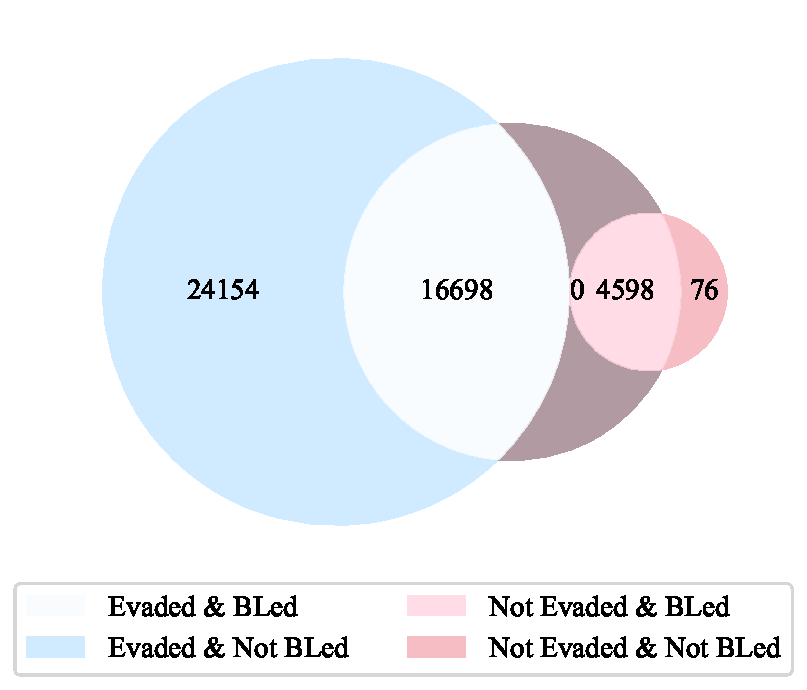
\includegraphics[width=\linewidth]{figs/venn_eval_3.pdf}
\caption{Venn Diagram describing the evasion from \spartacus and support from the anti-phishing ecosystem.}
\label{fig:venn_support}
% \vspace{-10pt}
\end{figure}

\begin{figure}
\centering
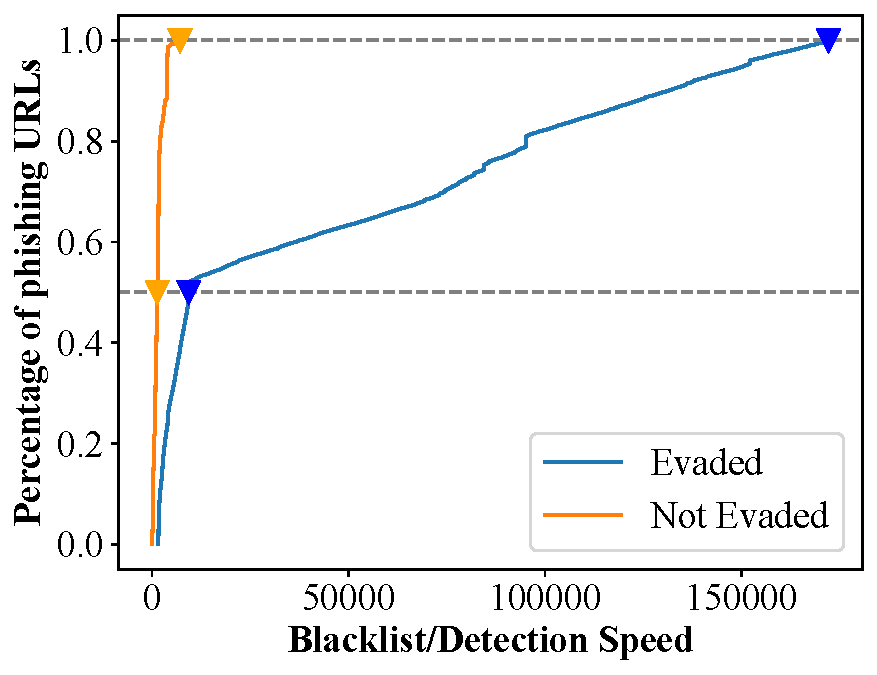
\includegraphics[width=\linewidth]{figs/evade_bl_time_total.pdf}
\caption{CDF of Blacklist/Detection time of current anti-phishing systems against phishing URLs evaded and not evaded by \spartacus.}
\label{fig:evade_bl_time}
% \vspace{-10pt}
\end{figure}